% Source: Code/ML_overlay/ir_rgb_registration/paper/ml_overlay_report_materials/ir_rgb_registration_report/figures/fig_raft_iteration_convergence.tex
\documentclass[tikz,border=10pt]{standalone}
\usepackage{pgfplots}
\pgfplotsset{compat=1.18}

\definecolor{Garnet}{RGB}{115,0,10}
\definecolor{Rose}{RGB}{204,46,64}
\definecolor{Atlantic}{RGB}{70,106,159}
\definecolor{Horseshoe}{RGB}{101,120,11}
\definecolor{Black90}{RGB}{54,54,54}
\definecolor{Black50}{RGB}{162,162,162}

\begin{document}
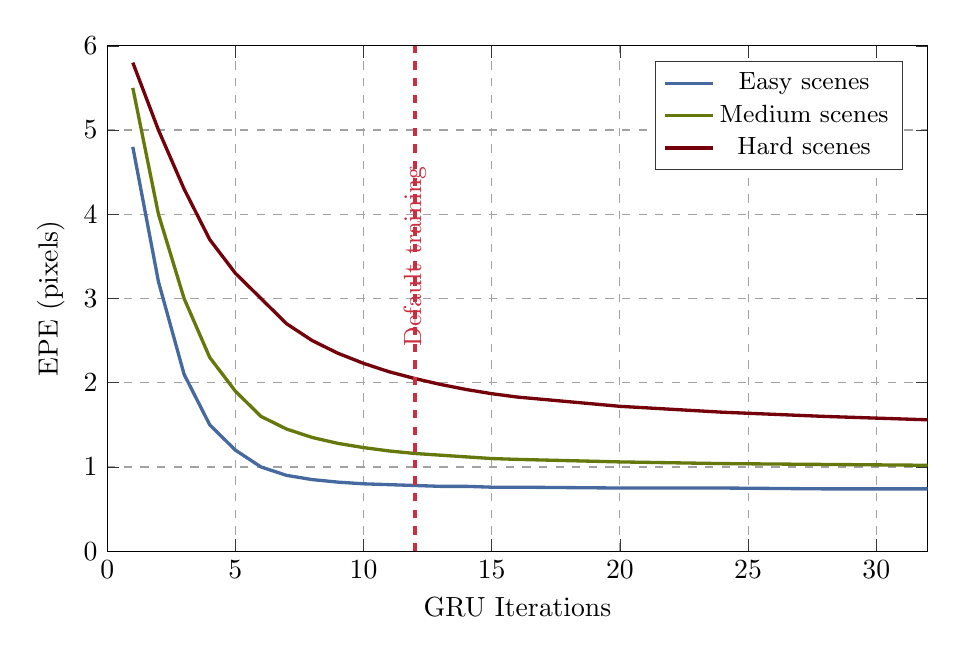
\begin{tikzpicture}
\begin{axis}[
    width=12cm,
    height=8cm,
    xlabel={GRU Iterations},
    ylabel={EPE (pixels)},
    xmin=0, xmax=32,
    ymin=0, ymax=6,
    grid=major,
    grid style={dashed,Black50},
    legend pos=north east,
    legend style={draw=Black90,fill=white,font=\small},
    tick style={Black90},
    every axis plot/.append style={thick,mark=none}
]

% Easy scenes (converges fast)
\addplot[Atlantic,line width=1.2pt] coordinates {
    (1,4.8) (2,3.2) (3,2.1) (4,1.5) (5,1.2) (6,1.0) (7,0.9) (8,0.85)
    (9,0.82) (10,0.80) (11,0.79) (12,0.78) (13,0.77) (14,0.77) (15,0.76)
    (16,0.76) (20,0.75) (24,0.75) (28,0.74) (32,0.74)
};
\addlegendentry{Easy scenes}

% Medium scenes
\addplot[Horseshoe,line width=1.2pt] coordinates {
    (1,5.5) (2,4.0) (3,3.0) (4,2.3) (5,1.9) (6,1.6) (7,1.45) (8,1.35)
    (9,1.28) (10,1.23) (11,1.19) (12,1.16) (13,1.14) (14,1.12) (15,1.10)
    (16,1.09) (20,1.06) (24,1.04) (28,1.03) (32,1.02)
};
\addlegendentry{Medium scenes}

% Hard scenes (converges slower)
\addplot[Garnet,line width=1.2pt] coordinates {
    (1,5.8) (2,5.0) (3,4.3) (4,3.7) (5,3.3) (6,3.0) (7,2.7) (8,2.5)
    (9,2.35) (10,2.23) (11,2.13) (12,2.05) (13,1.98) (14,1.92) (15,1.87)
    (16,1.83) (20,1.72) (24,1.65) (28,1.60) (32,1.56)
};
\addlegendentry{Hard scenes}

% Vertical line at iteration 12
\addplot[Rose,dashed,line width=1.5pt] coordinates {(12,0) (12,6)};
\node[Rose,font=\small,rotate=90] at (axis cs:12,3.5) {Default training};

\end{axis}
\end{tikzpicture}
\end{document}
